\section{Hardware Implementation}
\label{sec:implementation}

We have built a 20-node FlashBoost cluster to explore the capabilities of the
architecture. Figure~\ref{fig:bluedbmcluster} shows the photo of our
implementation.

\begin{figure}[ht]
	\begin{center}
	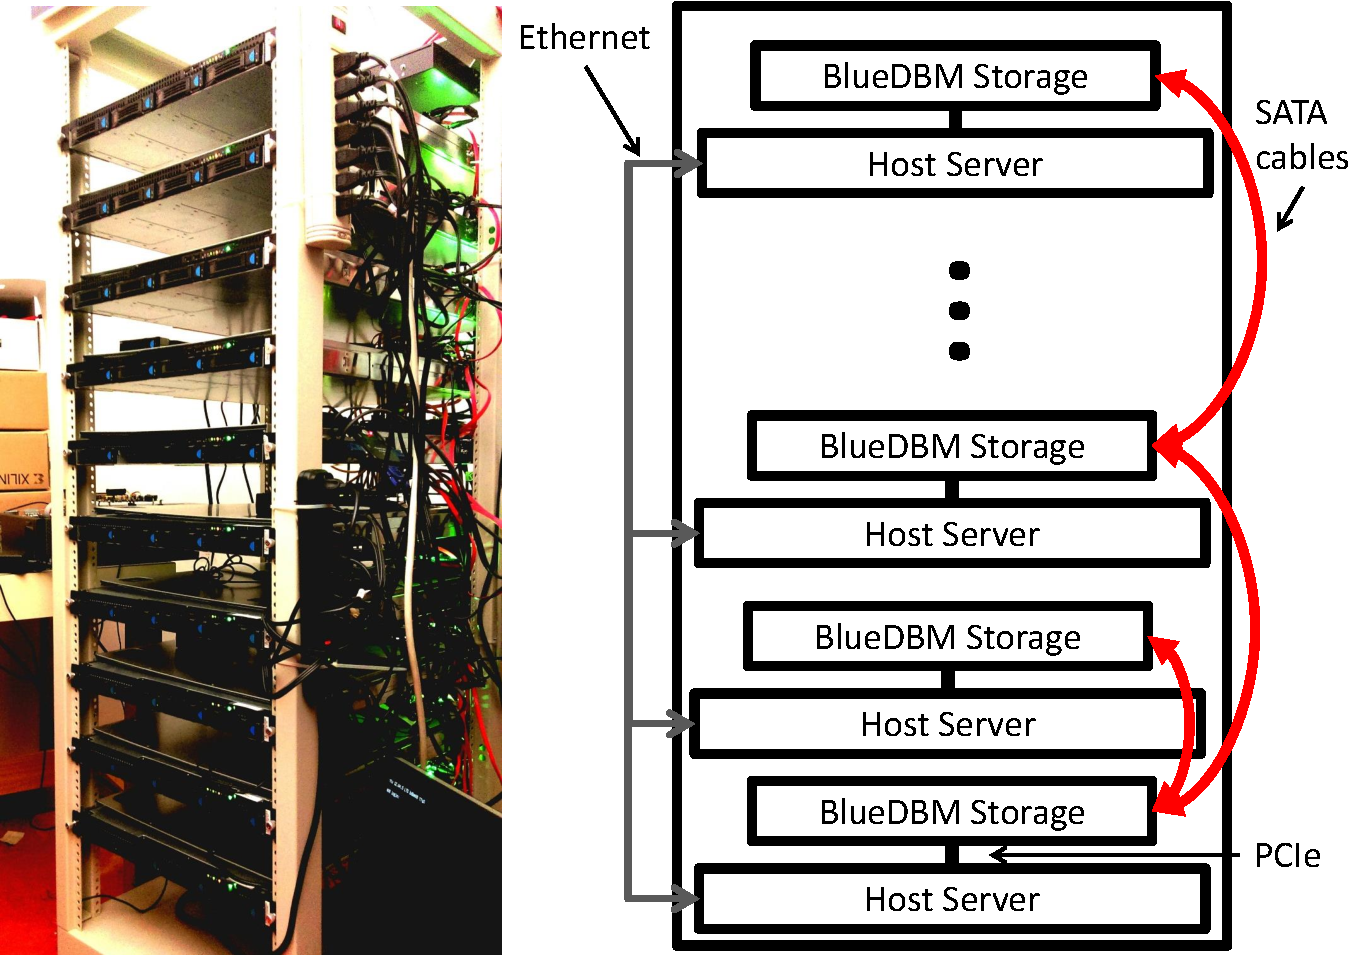
\includegraphics[width=0.4\paperwidth]{figures/rackserver-crop.pdf}
	%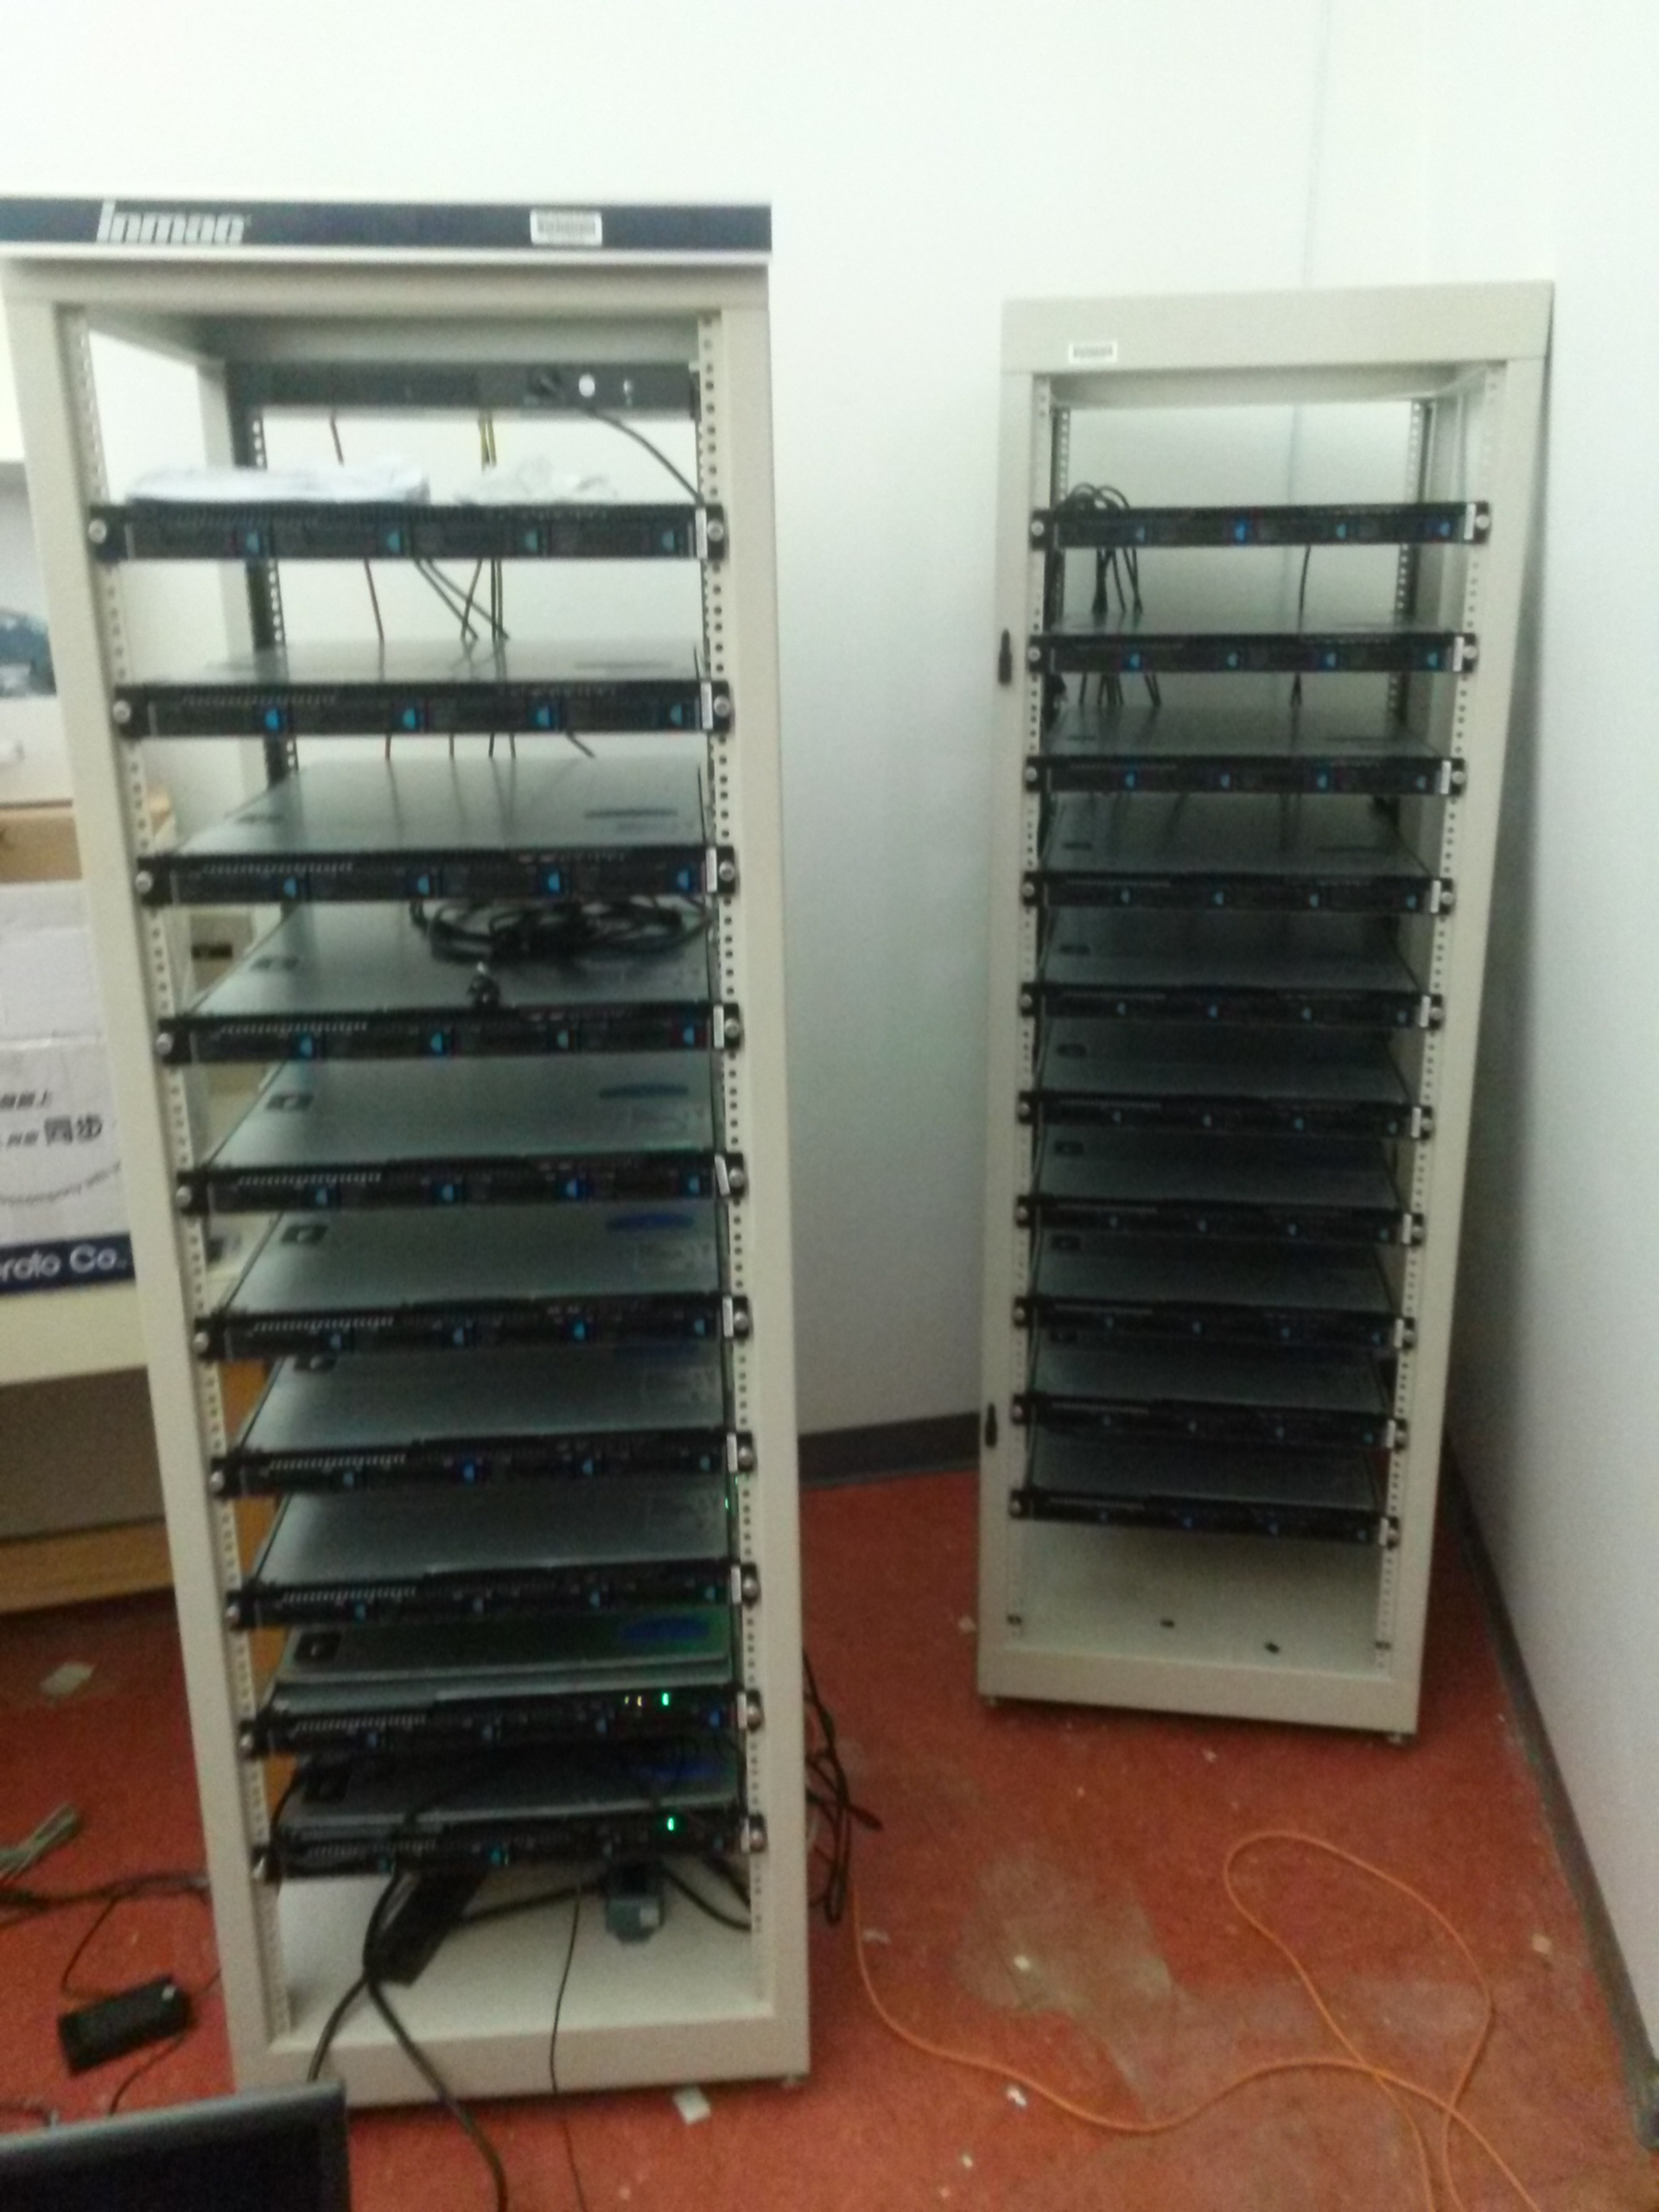
\includegraphics[width=0.3\paperwidth]{figures/rack.jpg}
	\caption{A 20-node FlashBoost Cluster}
	\label{fig:bluedbmcluster}
	\end{center}
\end{figure}

%\begin{figure}[ht!]
%	\begin{tabular}{cc}
%
%	\multirow{2}{*}{
%	\begin{minipage}[c]{.20\textwidth}
%	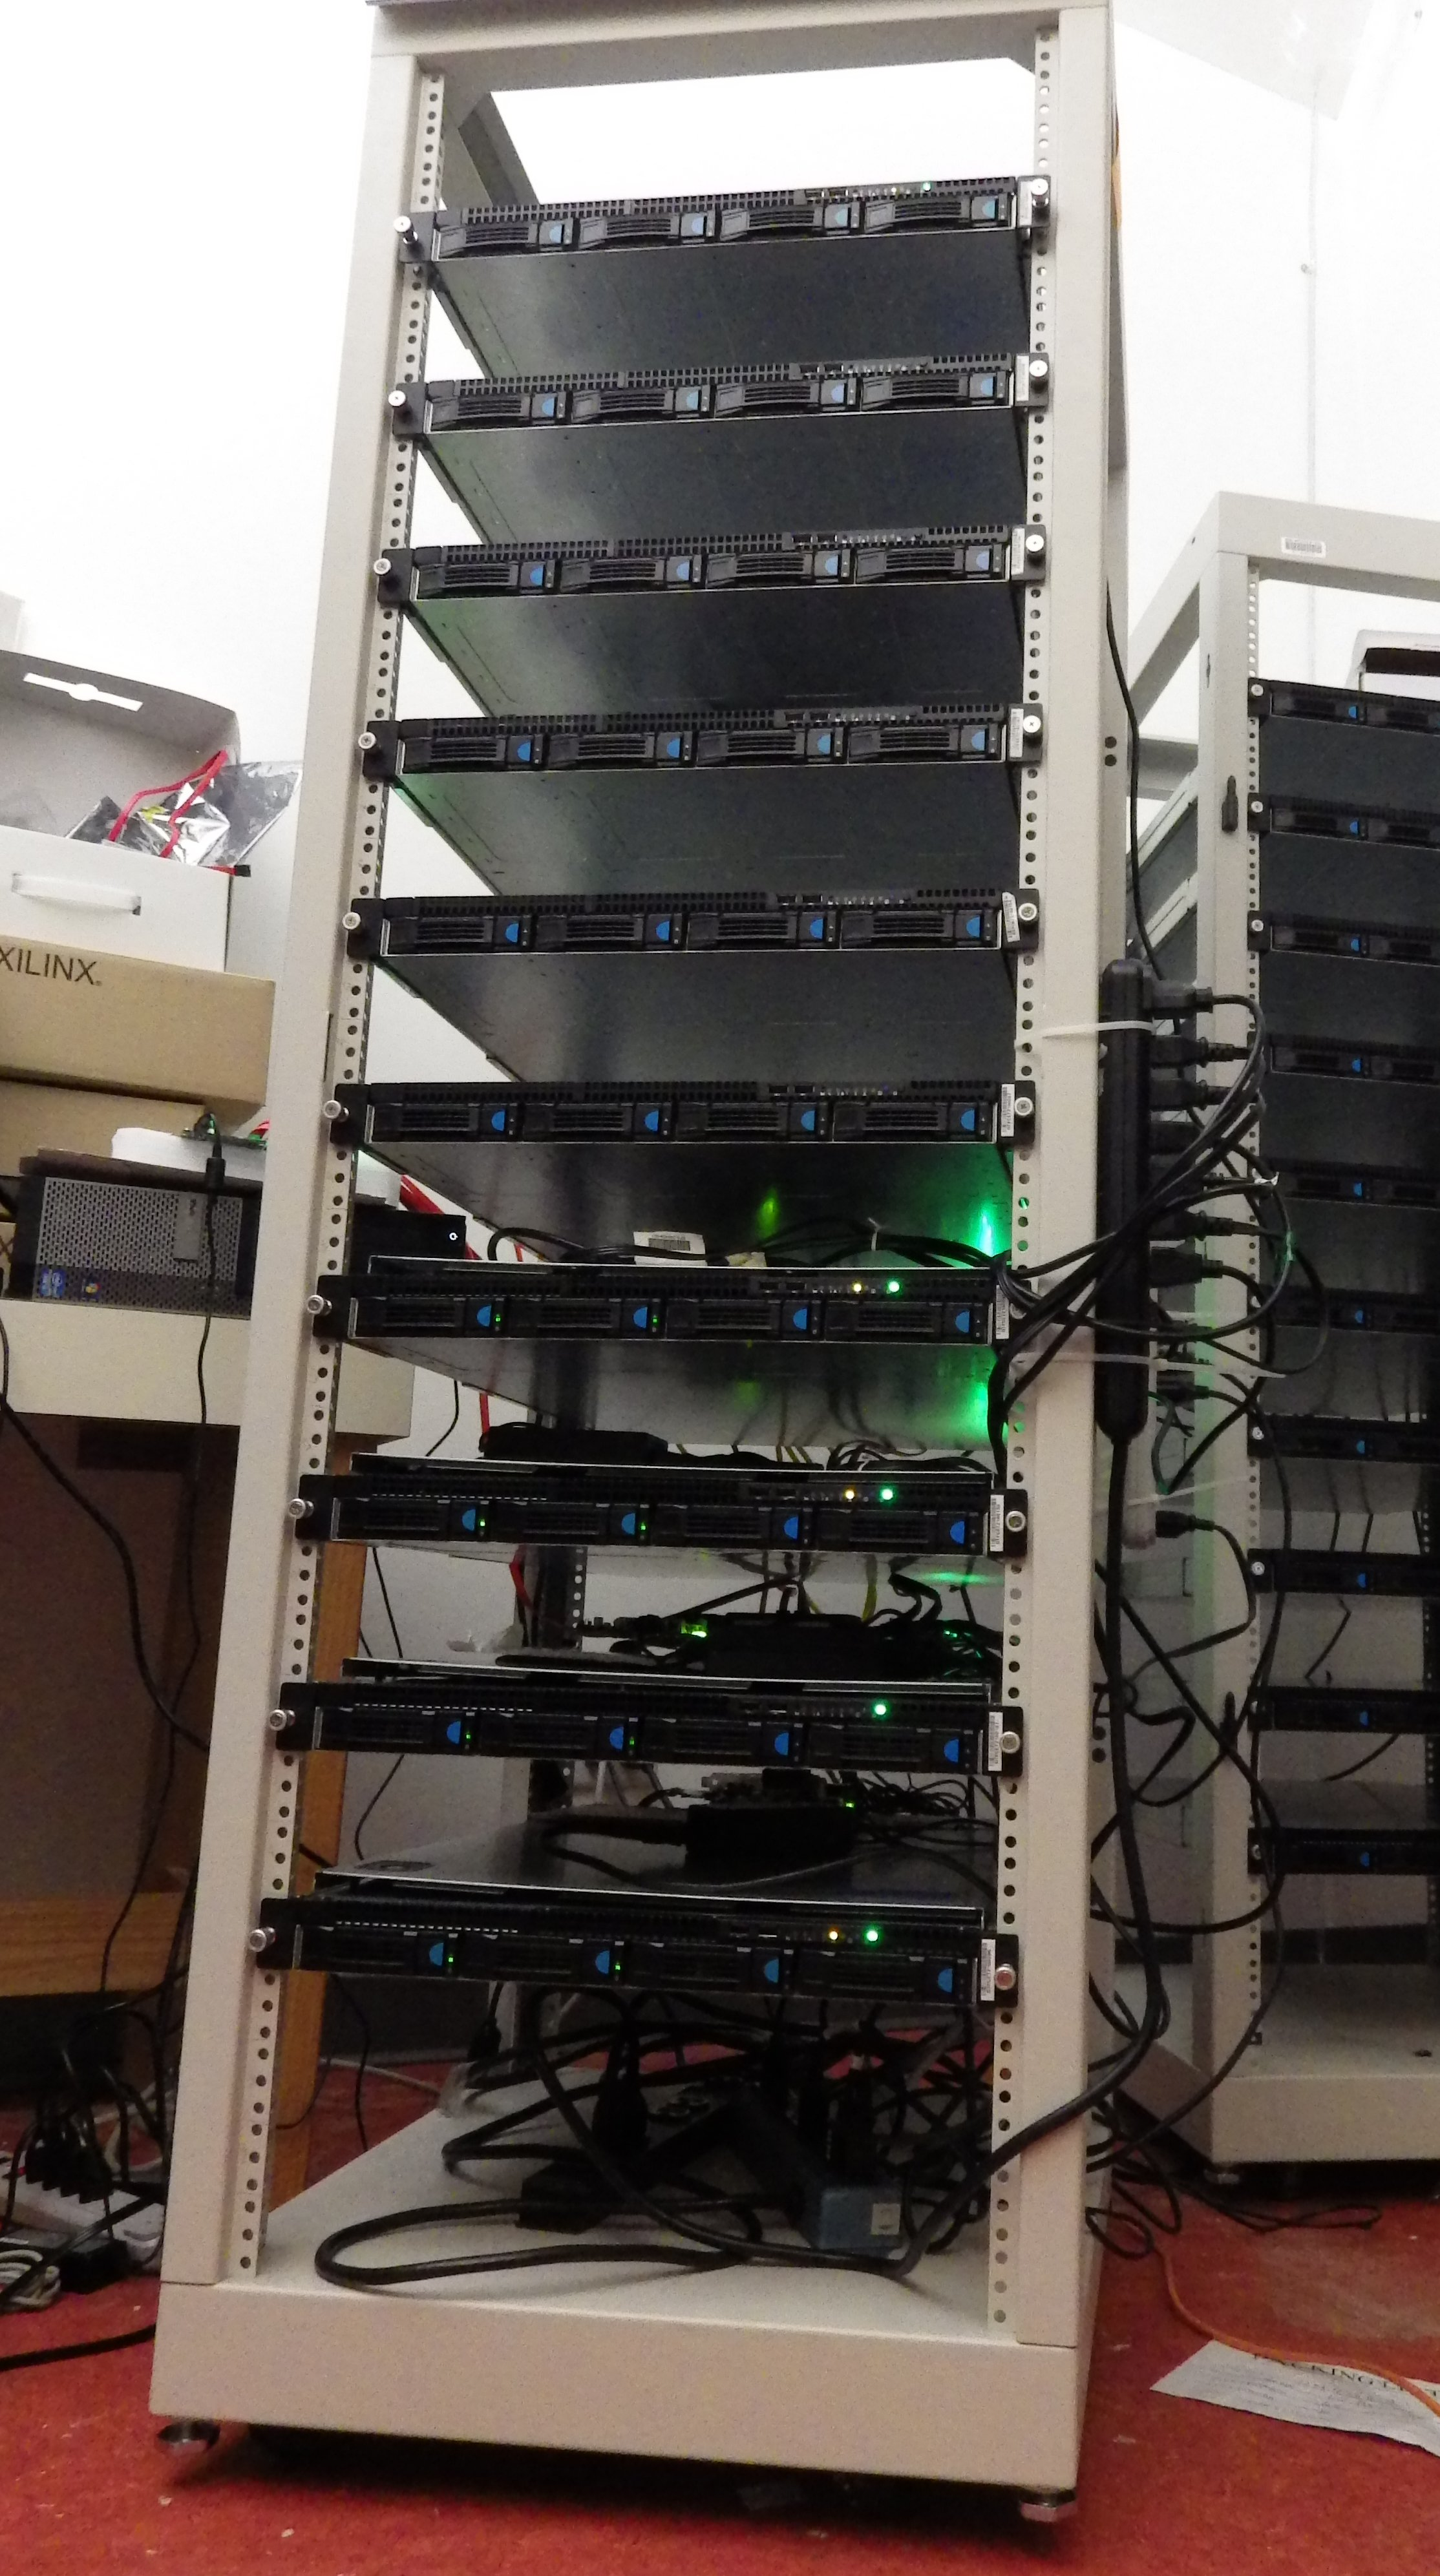
\includegraphics[width=\textwidth]{figures/rackserver2.jpg}
%	\caption{One of the two 10-node FlashBoost Racks}
%	\label{fig:bluedbmcluster}
%	\end{minipage}
%	}
%	& 
%	\begin{minipage}[c]{.20\textwidth}
%	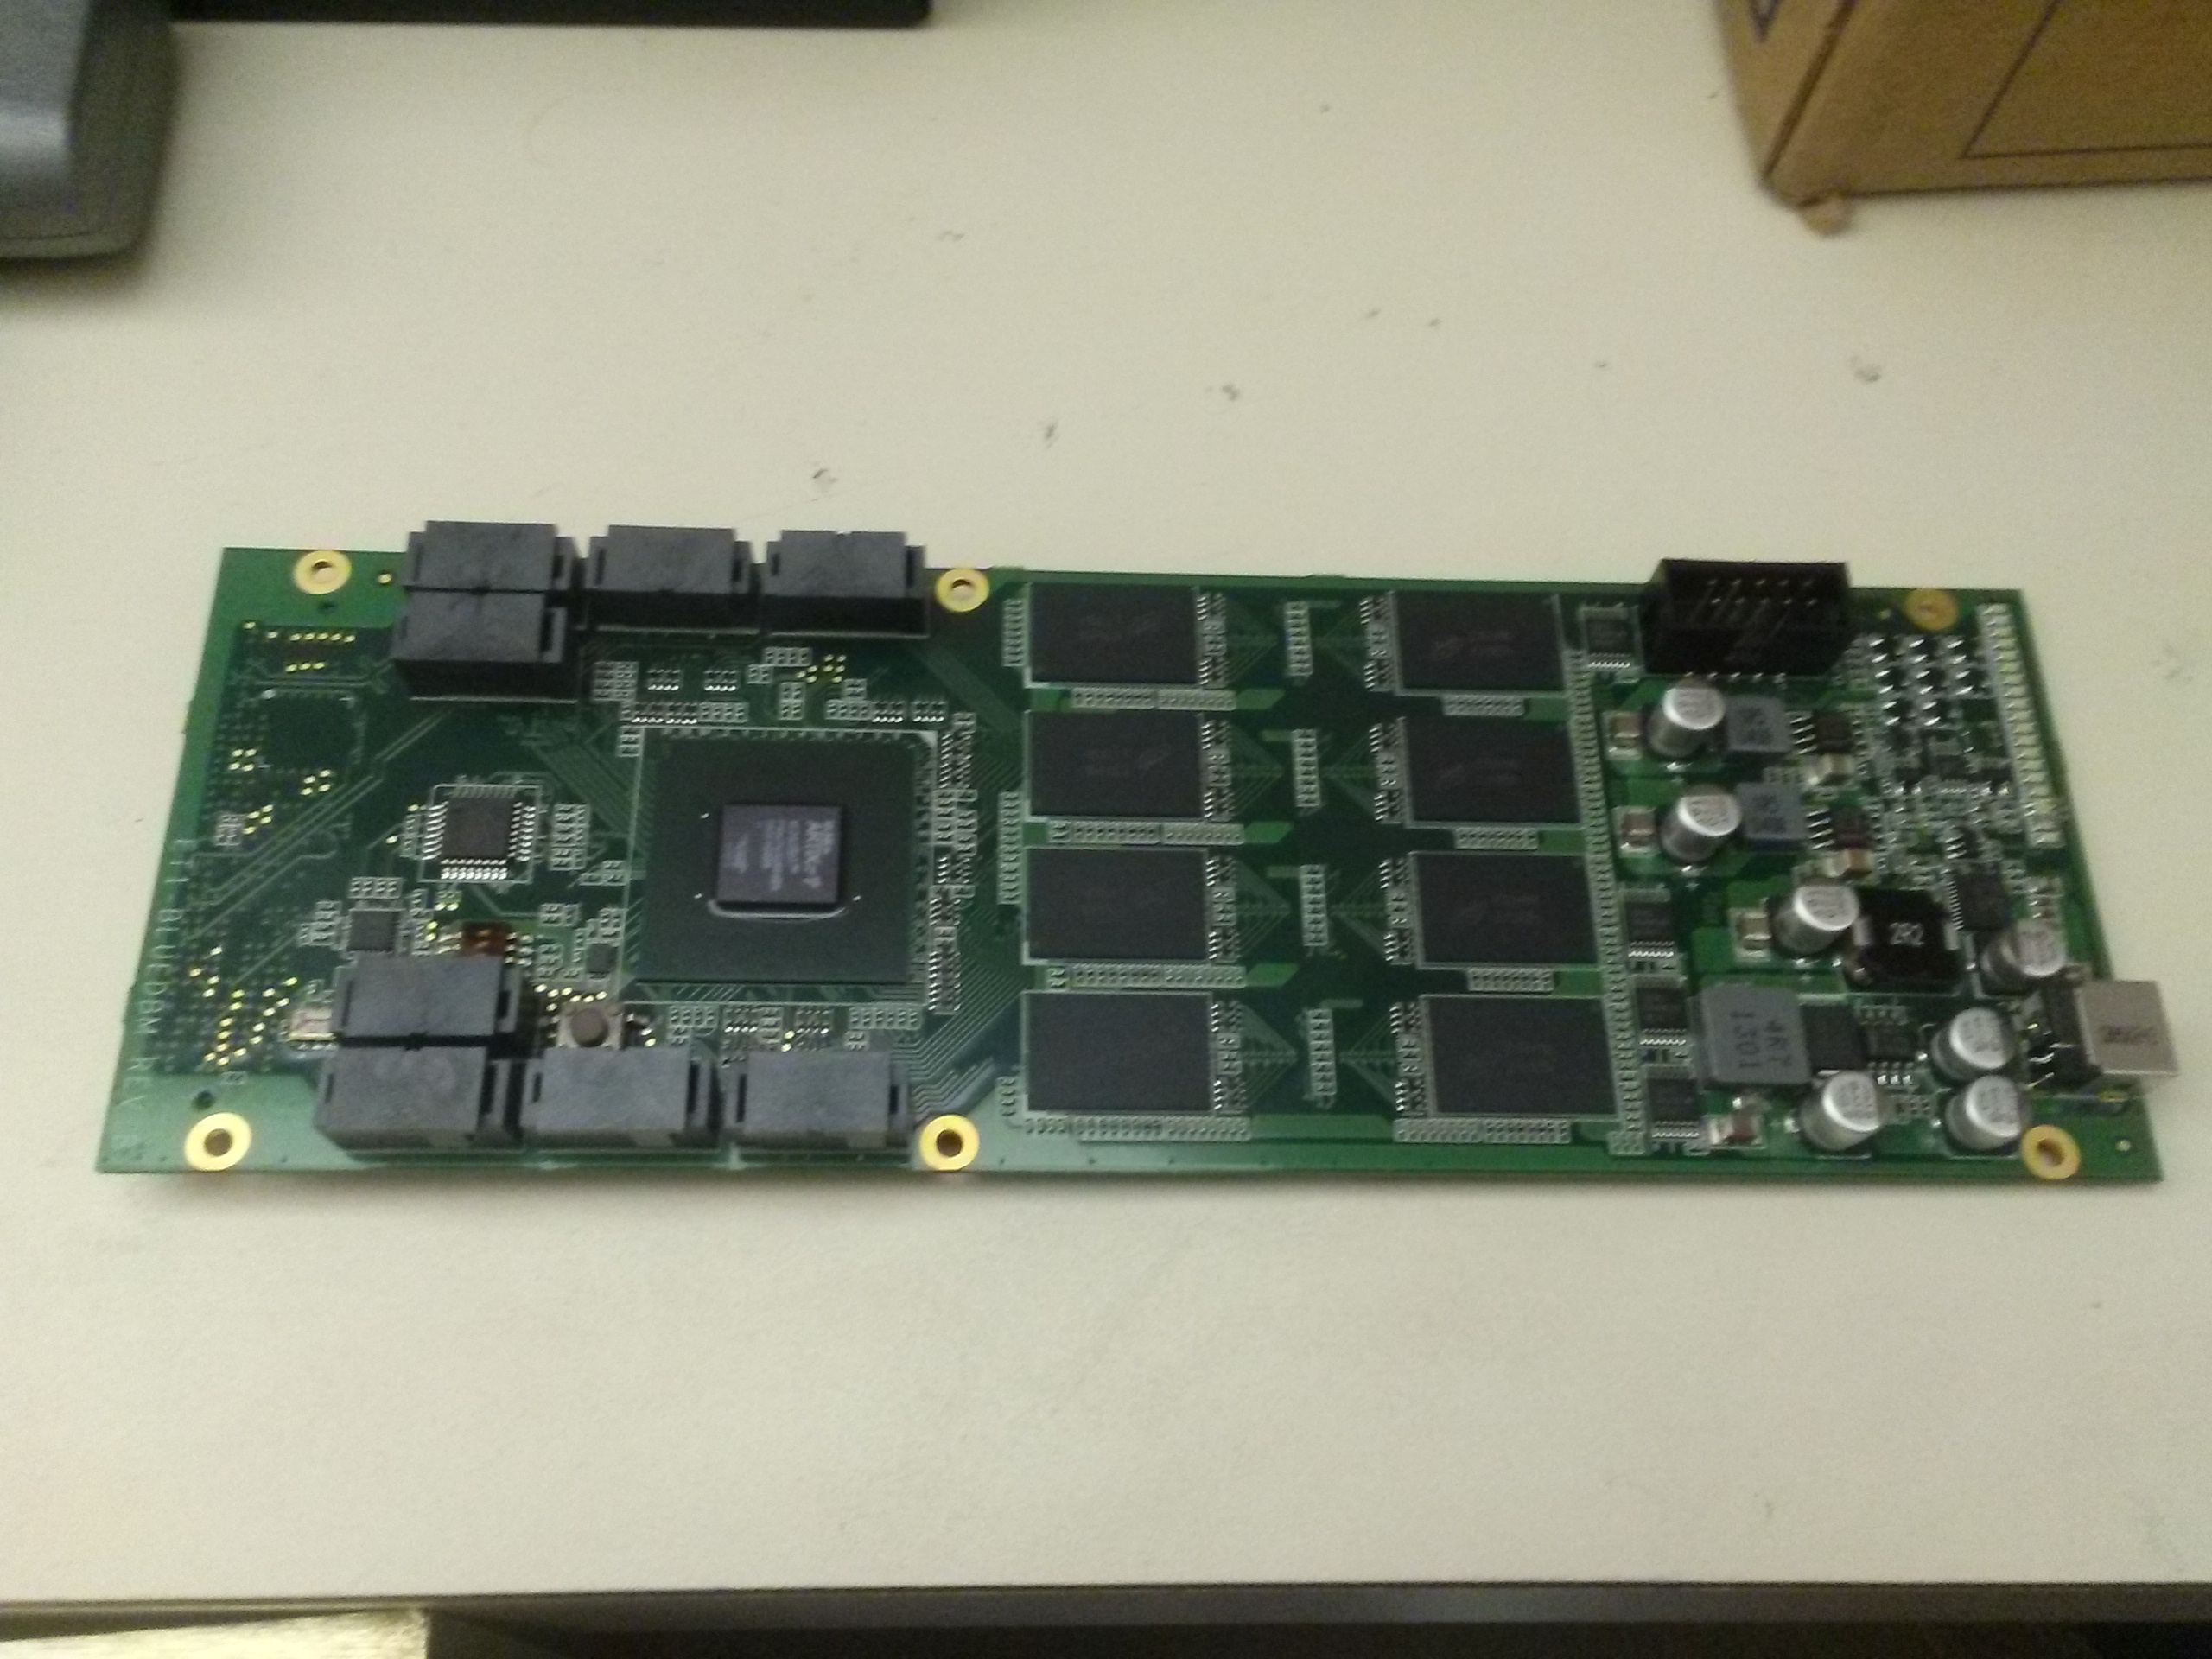
\includegraphics[width=\textwidth]{figures/flashboard.jpg}
%	\caption{A Custom Flash Card}
%	\label{fig:flashboard}
%	\end{minipage} \\
%	&
%	\begin{minipage}[c]{.20\textwidth}
%	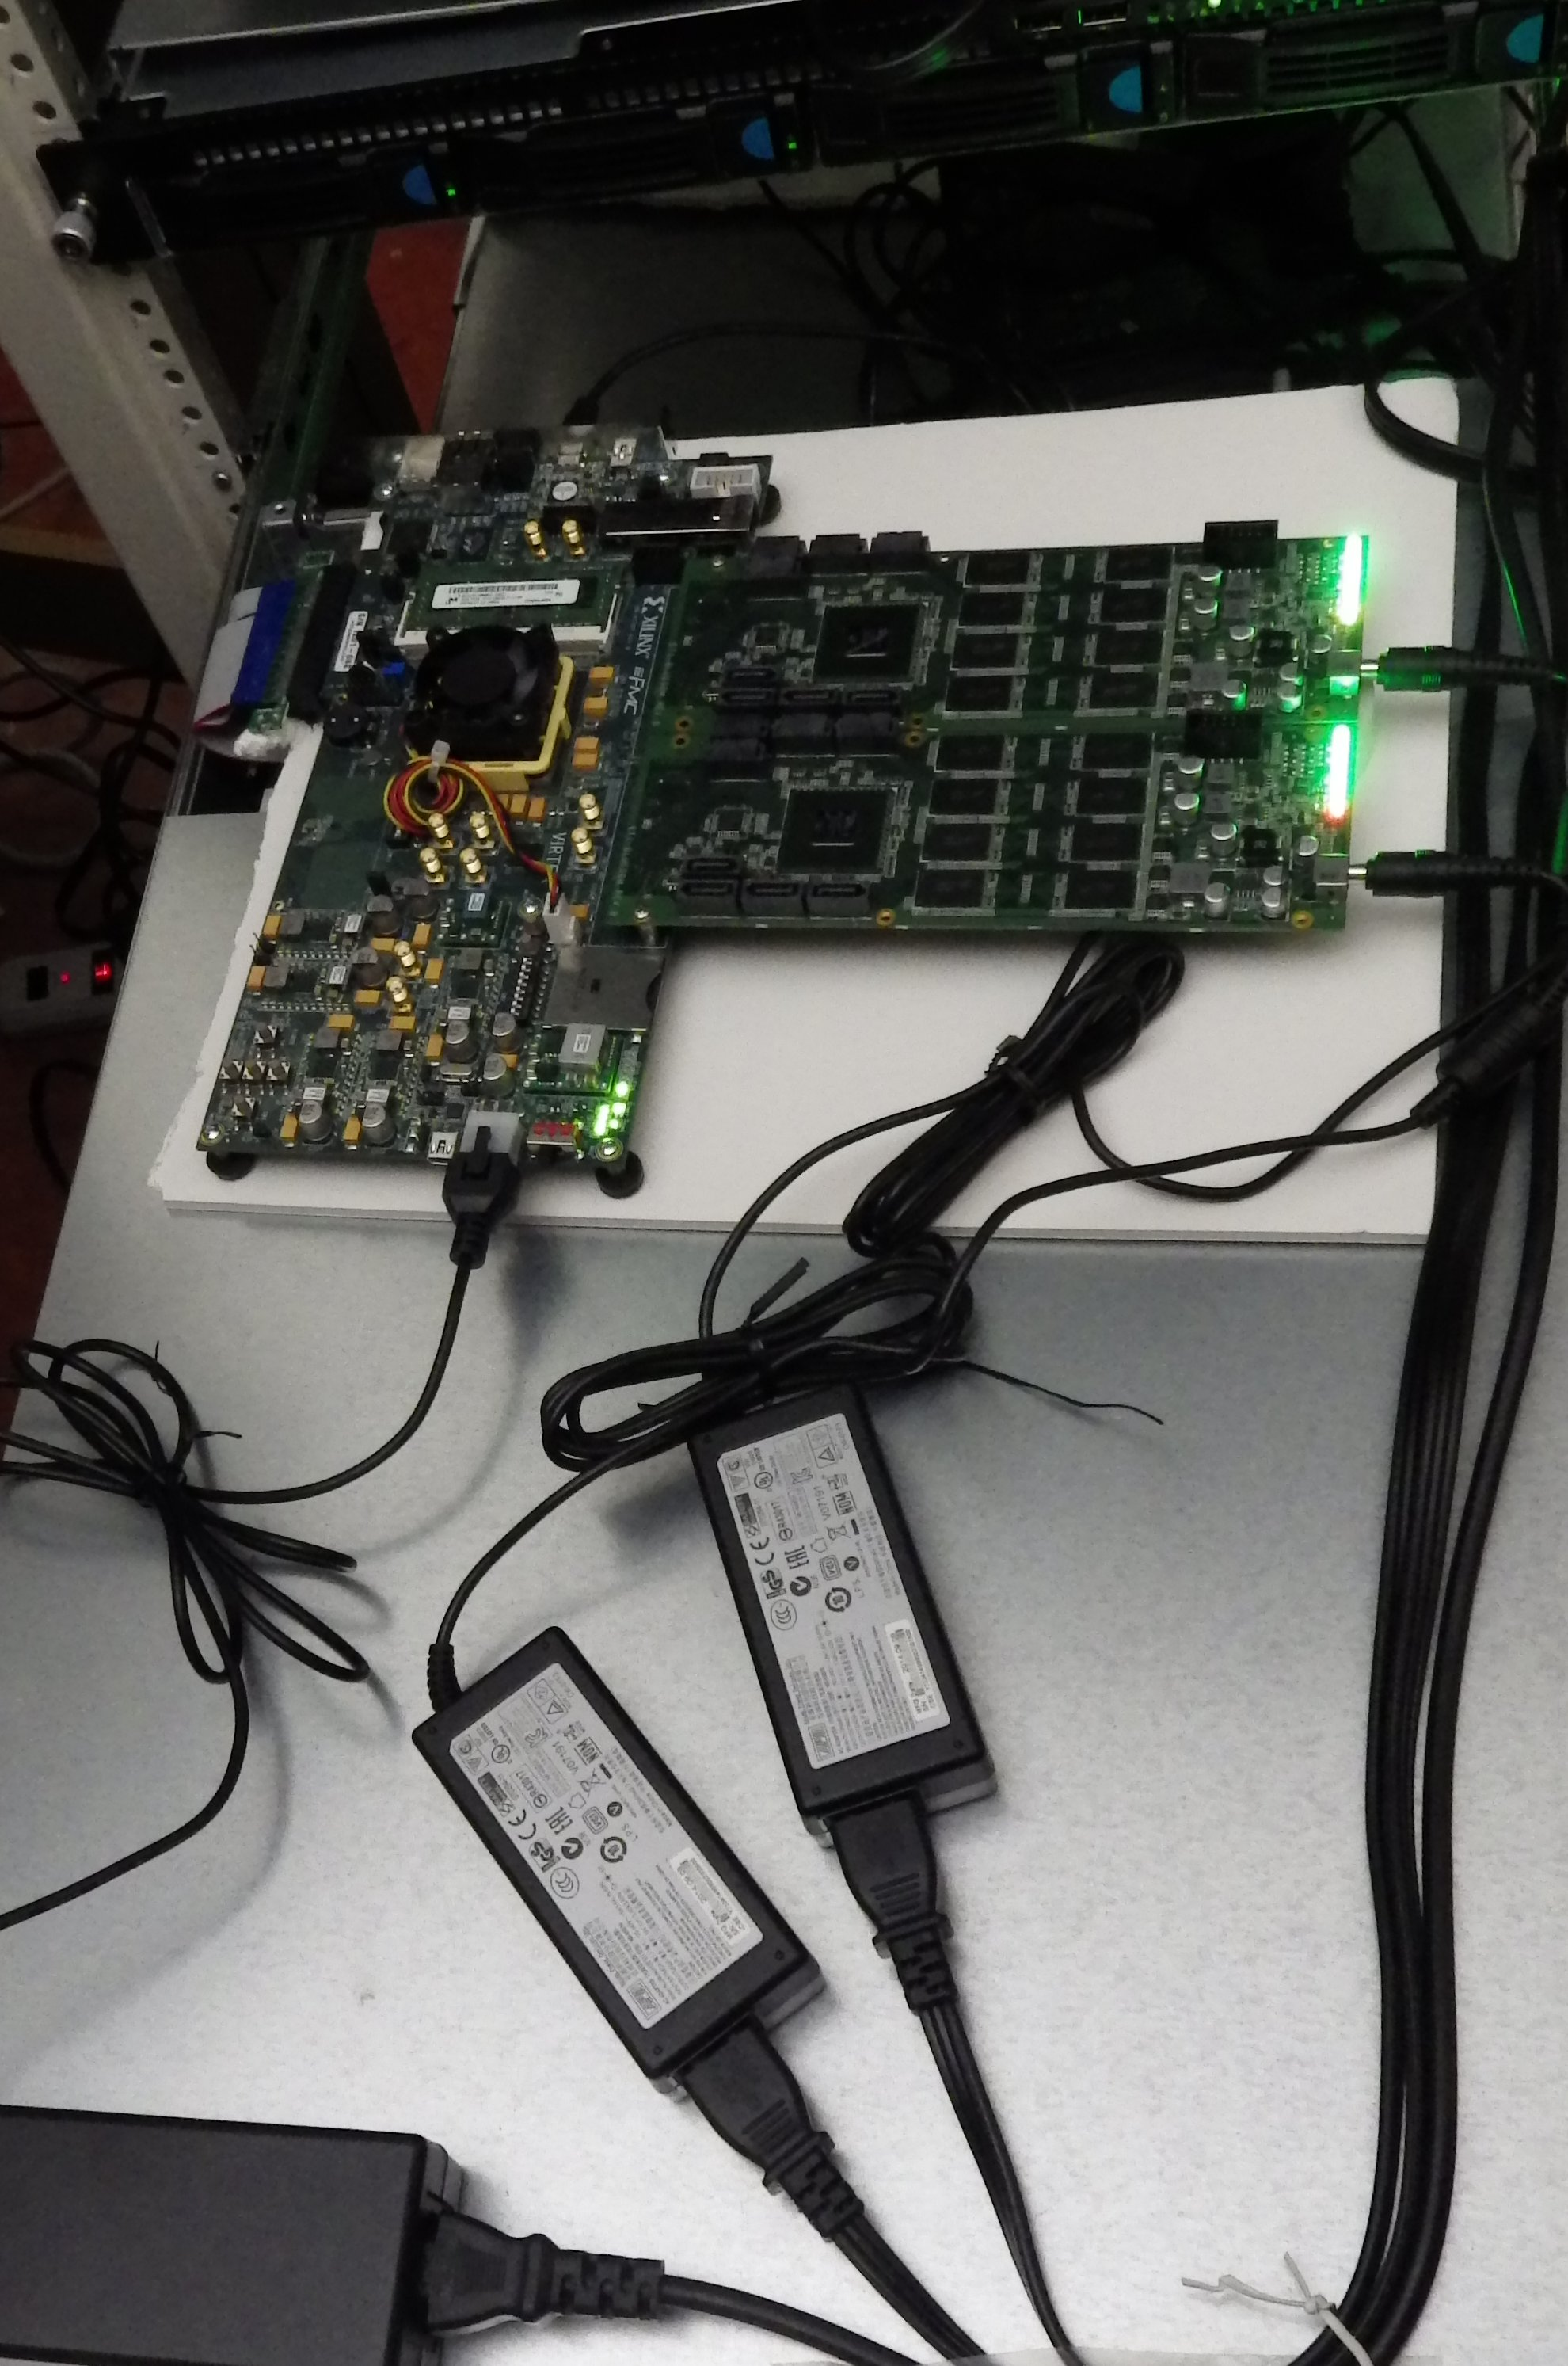
\includegraphics[width=\textwidth]{figures/racknode.jpg}
%	\caption{A FlashBoost Rack Node}
%	\label{fig:flashrack}
%	\end{minipage}
%	\end{tabular}
%\end{figure}
%\begin{figure}[ht]
%	\begin{center}
%	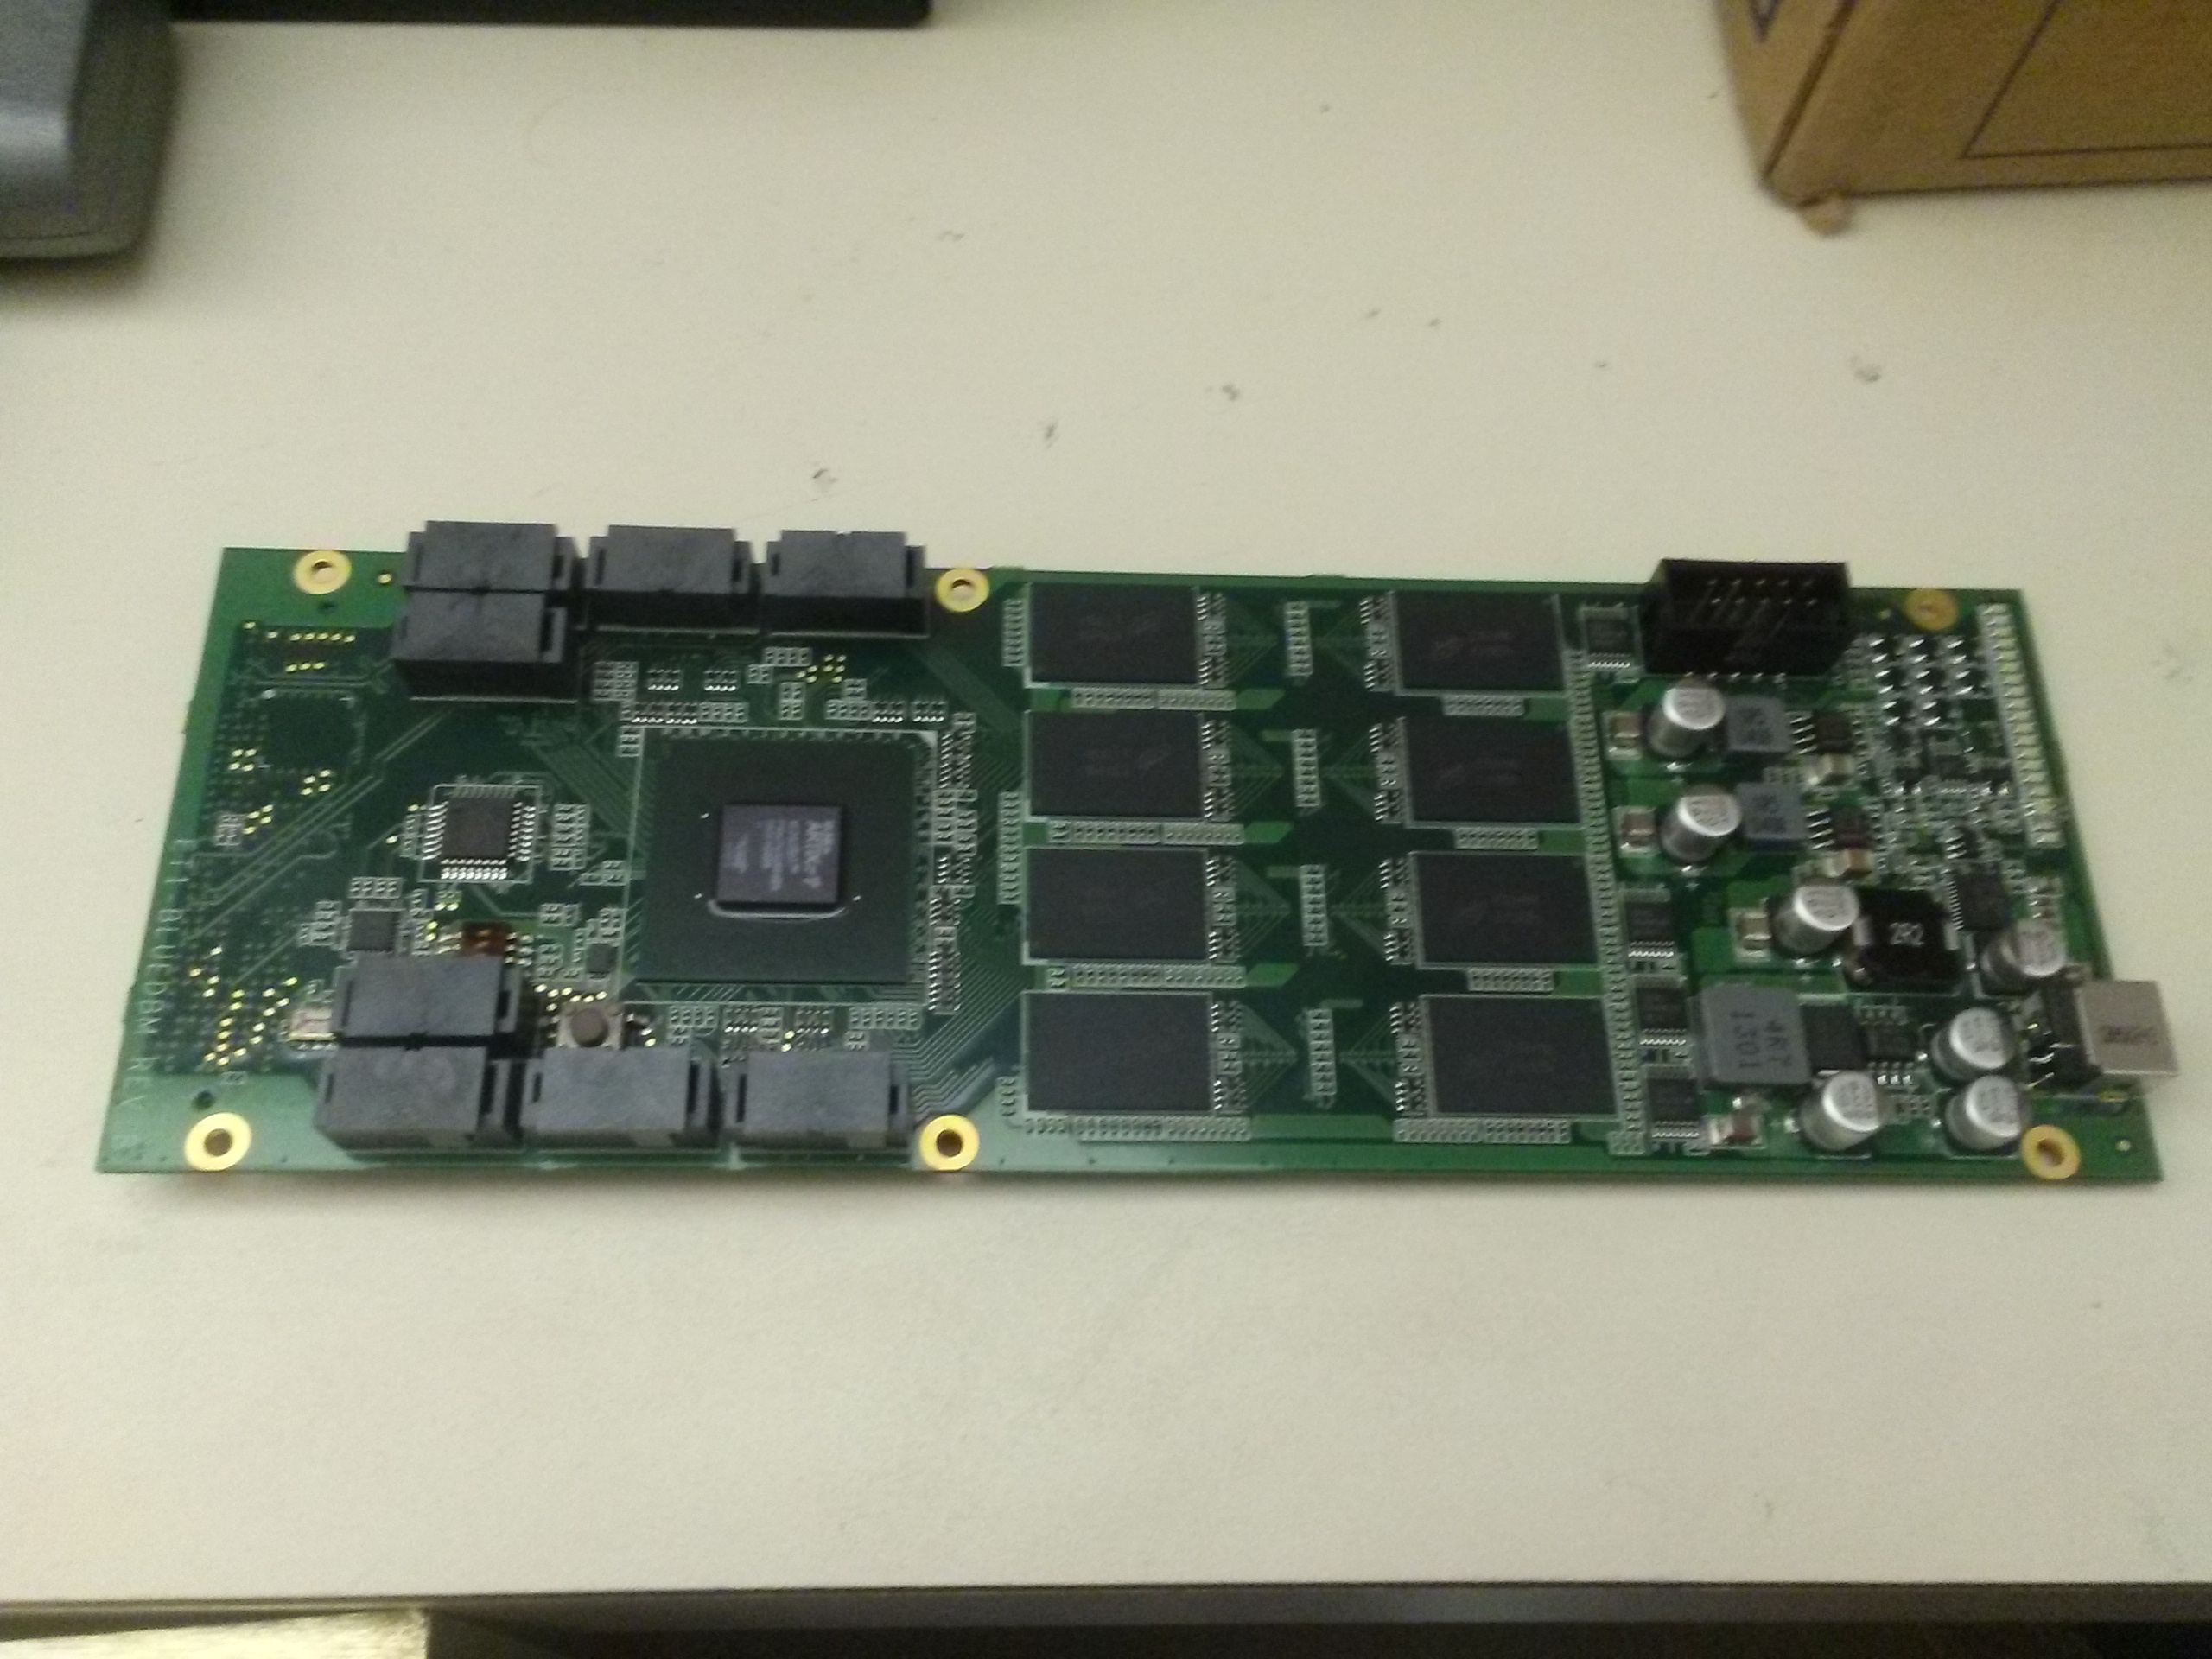
\includegraphics[width=0.4\textwidth]{figures/flashboard.jpg}
%	\caption{A Custom-Built Flash Board with 512GB of NAND Flash}
%	\label{fig:flashboard}
%	\end{center}
%\end{figure}
%	\subfloat[One of the two 10-node FlashBoost Racks]
%		{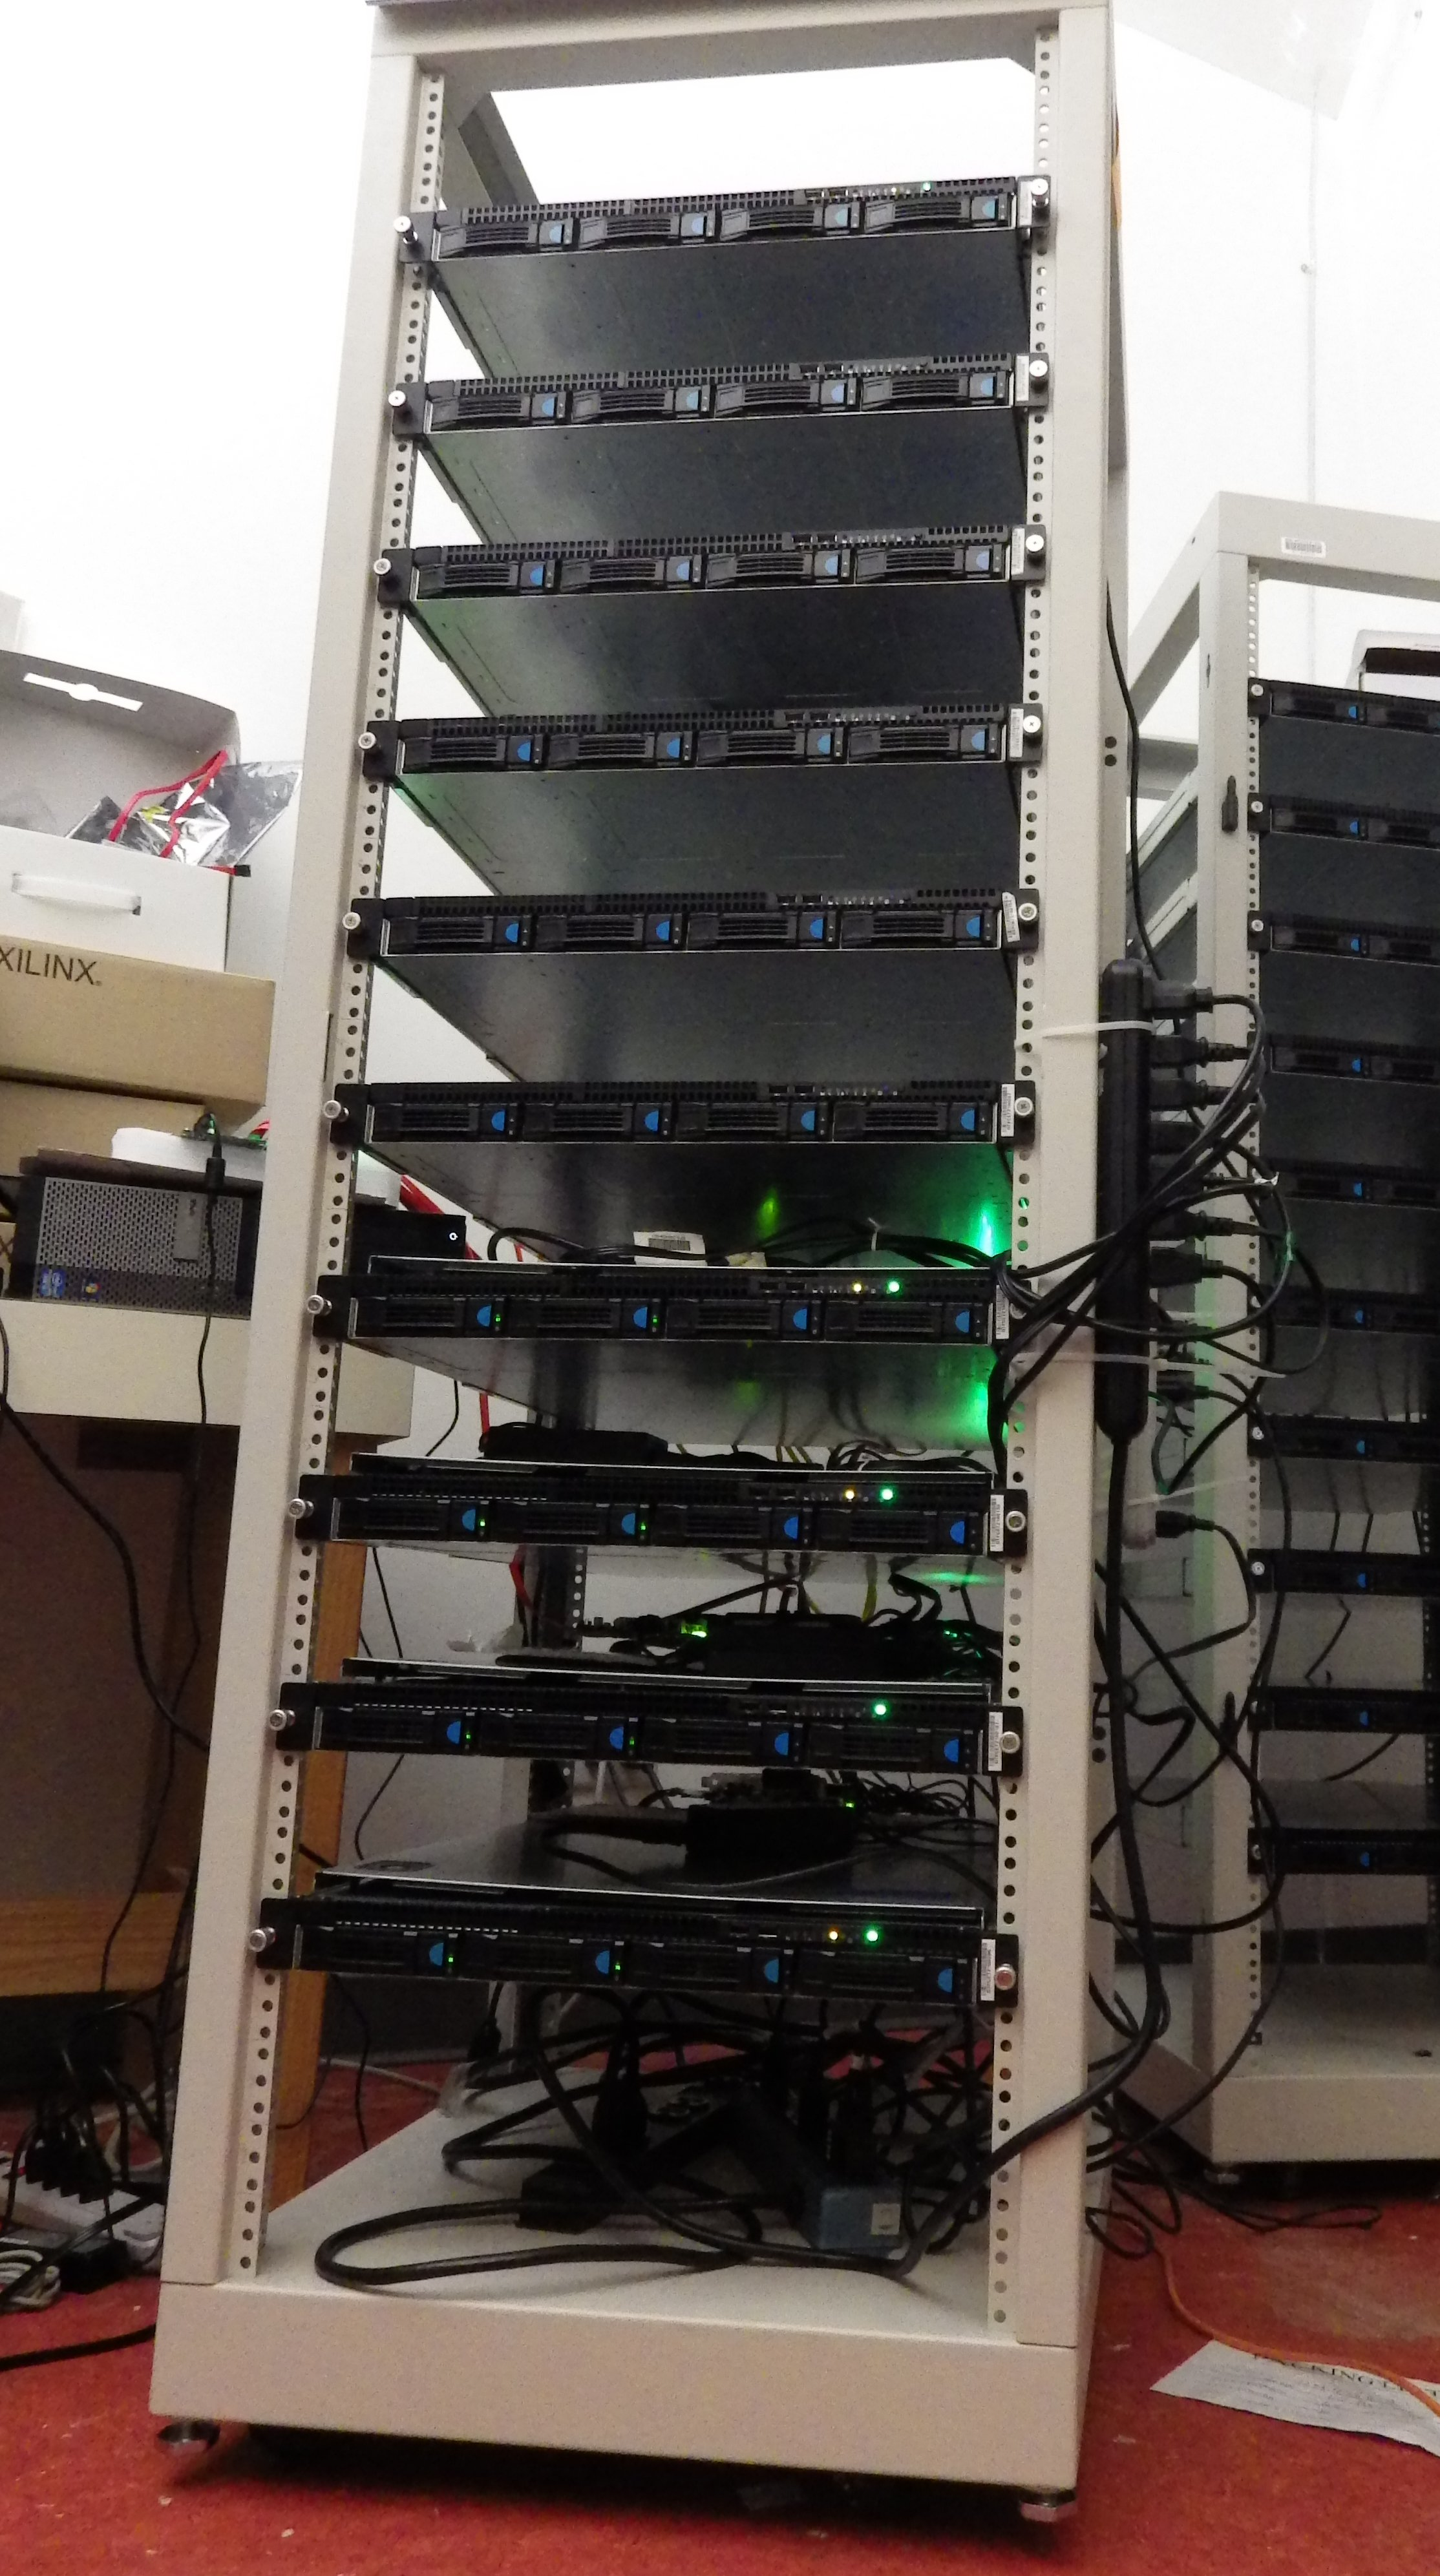
\includegraphics[width=0.22\textwidth]{figures/rackserver2.jpg}}
%	} 

In our implementation of FlashBoost, we have used a Field Programmable Gate
Array (FPGA) to implement the in-store processor and also the flash, host and
network controllers. However, the FlashBoost Architecture should not be limited
to an FPGA-based implementation.  Development of FlashBoost was done in the
high-level hardware description language Bluespec. It is possible to develop in-store processors in any hardware description language, as long as they conform to the interface exposed by the FlashBoost system services. Most of the interfaces are latency-insensitive FIFOs with backpressure. Bluespec provides a lot of support for such interfaces, making in-store accelerator development easier.

The cluster consists of 20 rack-mounted Xeon servers, each with a Xilinx
VC707 FPGA development board connected via a PCIe connection. Each VC707 board
hosts two custom-built flash boards with SATA connectors. The VC707 board,
coupled with two custom flash boards is mounted on top of each server.
The host servers run the Ubuntu distribution of Linux.
Figure~\ref{fig:bluedbmnode} shows the components of a single node.
One of the servers also had a 512GB Samsung M.2 PCIe SSD for performance
comparisons.

We used Connectal~\cite{connectal} and its PCIe Gen 1 implementation for the
host link. This PCIe implementation caps our performance at 1.6GB/s reads and
1GB/s writes, which is a reasonable performance for a commodity flash storage
device. In the future we will also explore the benefits of a faster host link
including later generation PCIe links.

\begin{figure}[ht]
	\begin{center}
	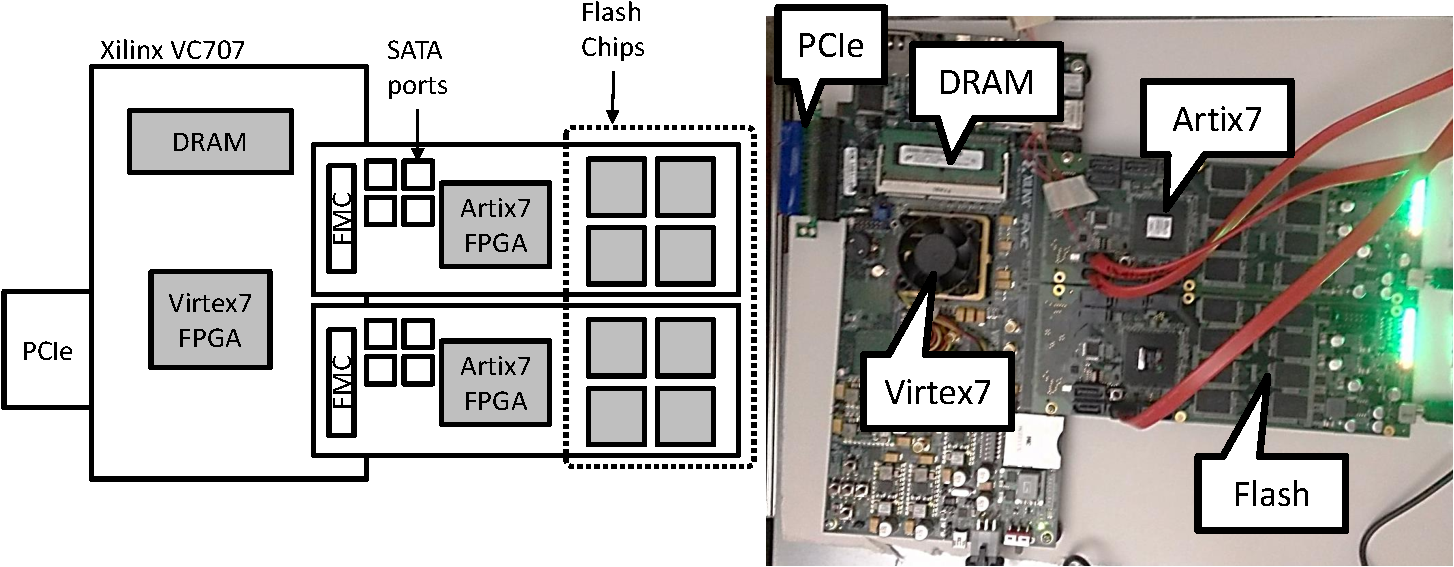
\includegraphics[width=0.5\textwidth]{figures/racknode-crop.pdf}
	\caption{A FlashBoost Storage Node}
	\label{fig:bluedbmnode}
	\end{center}
\end{figure}


\subsection{Custom Flash Board}

%\begin{figure}[ht]
%	\begin{center}
%	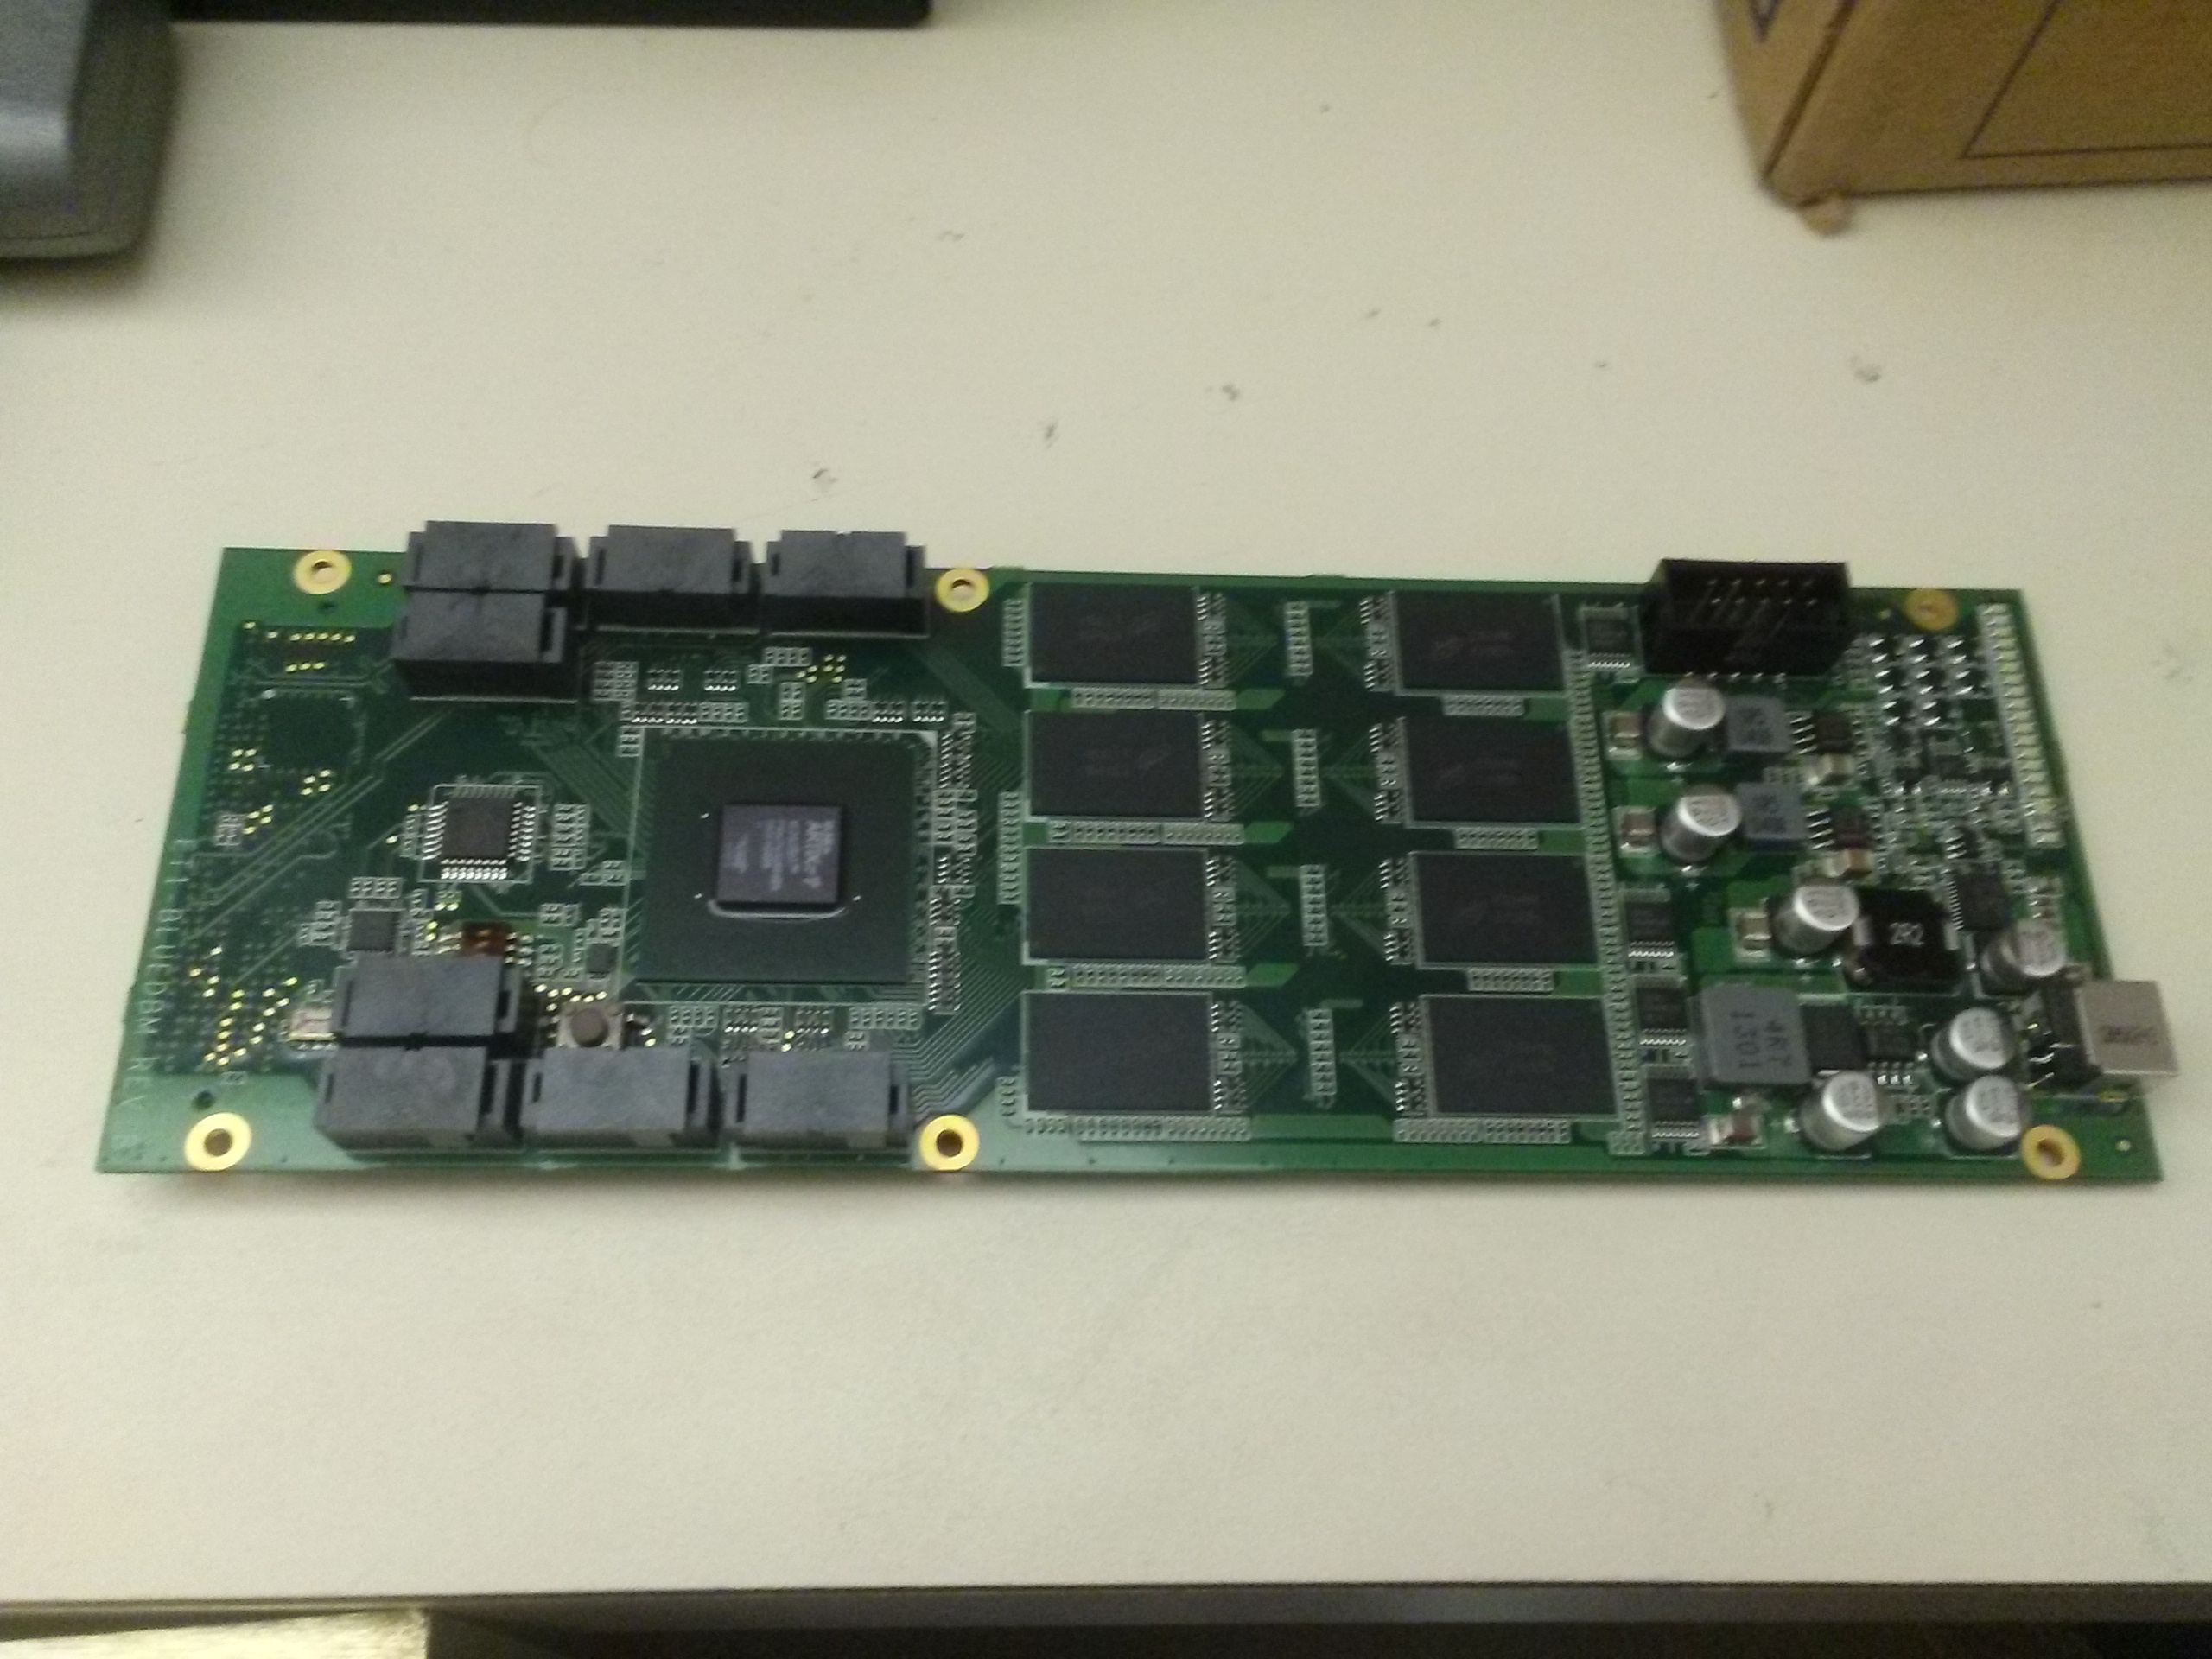
\includegraphics[width=0.4\textwidth]{figures/flashboard.jpg}
%	\caption{A Custom-Built Flash Board with 512GB of NAND Flash}
%	\label{fig:flashboard}
%	\end{center}
%\end{figure}

We have designed and built a high-capacity custom flash board with high-speed
serial connectors, with the help of Quanta Inc., and Xilinx Inc.

Each flash card has 512GBs of NAND flash storage and a Xilinx Artix 7 chip, and
plugs into the host FPGA development board via the FPGA Mezzanine Card (FMC)
connector. The flash controller and Error Correcting Code (ECC) is implemented
on this Artix chip, providing the Virtex 7 FPGA chip on the VC707 a logical
error-free access into flash. The communication between the flash board and the
Virtex 7 FPGA is done by a 4-lane aurora channel, which is implemented on the
GTX/GTP serial transceivers included in each FPGA. This channel can sustain up
to 3.3GB/s of bandwidth at 0.5$\mu s$ latency.
The flash board also hosts 8 SATA connectors, 4 of
which pin out the high-speed serial ports on the host Virtex 7 FPGA,
and 4 of whch pin out the high-speed serial ports on the Artix 7 chip.
The serial ports are capable of 10Gbps and 6.6Gbps of bandwidth, respectively.

\subsection{Network Infrastructure}

In our FlashBoost implementation, the link is implemented over the
low-latency serial transceivers.  By
implementing routing in the hardware and using a very low-latency network
fabric, we were able to achieve very high performance, with less than 0.5$\mu s$ of
latency per network hop, and near 10Gbps of bandwidth per link. Our
implementation has a network fan-out of 8 ports per storage node, so the
aggregate network bandwidth available to a node reaches up to 8GB/s, including
packet overhead.

\subsection{Software Interface}

Our host interface was implemented using Connectal~\cite{connectal}, a
hardware-software codesign framework built by Quanta Research.
Connectal reads the interface definition file written by the programmer and
generates glue logic between hardware and software. Connectal automatically
generates RPC-like interface from developer-provided interface specification, as
well as a memory-mapped DMA interface for high bandwidth data transfer.
Connectal provides a PCIe Gen 1 endpoint and driver pair, and provides up to
1.6GB/s DMA read to host DRAM bandwidth and 1GB/s of DMA write from host DRAM
bandwidth. 

Reading or writing data from the host buffers were done by DMA read/write
engines implemented in the Connectal framework. In our FlashBoost
implementation, there are four read engines and four write engines each, in
order to more easily make maximum use of the PCIe bandwidth. 



